\documentclass[a4paper]{beamer}
\usepackage[spanish]{babel}
\usepackage[utf8]{inputenc}
\usepackage{graphicx}
\usepackage{biblatex}
\usepackage{enumerate}
\usepackage{csquotes}
\usepackage{braket}
\usepackage{amsmath}
\usepackage{pifont}

\title{Modos rotacionales y vibracionales en moléculas}
\author{José Soto García}
\begin{document}
\maketitle

%DIAPOSITIVA 2
\begin{frame}{La molécula como un sólido rígido}
\framesubtitle{Un poco de mecánica clásica}
  Para un sólido poliatómico se define el tensor de inercia $\tilde I$ como:
  \[\small{
\tilde{I}=\begin{pmatrix}
\displaystyle\sum_{\alpha}m_{\alpha}\left(x^2_{\alpha,2}+x^2_{\alpha,3}\right) & -\displaystyle\sum_{\alpha}m_{\alpha}x_{\alpha,1}x_{\alpha,2} & -\displaystyle\sum_{\alpha}m_{\alpha}x_{\alpha,1}x_{\alpha,3} \\\\
-\displaystyle\sum_{\alpha}m_{\alpha}x_{\alpha,2}x_{\alpha,1} & \displaystyle\sum_{\alpha}m_{\alpha}\left(x^2_{\alpha,1}+x^2_{\alpha,3}\right) &-\displaystyle\sum_{\alpha}m_{\alpha}x_{\alpha,2}x_{\alpha,3} \\\\
-\displaystyle\sum_{\alpha}m_{\alpha}x_{\alpha,3}x_{\alpha,1} & -\displaystyle\sum_{\alpha}m_{\alpha}x_{\alpha,3}x_{\alpha,2} & \displaystyle\sum_{\alpha}m_{\alpha}\left(x^2_{\alpha,1}+x^2_{\alpha,2}\right) \end{pmatrix}}
\]

La energía cinética rotacional del sistema se obtiene como
$$T_{rot}=\frac{1}{2}\sum_{i,j}I_{ij}\omega_i\omega_j$$

\end{frame}

%DIAPOSITIVA 3
\begin{frame}{La molécula como un sólido rígido}
\framesubtitle{Un poco de mecánica clásica}
Si diagonalizamos el tensor de inercia
$$\tilde I = \begin{pmatrix}
I_a & 0 & 0\\
0 & I_b & 0\\
0 & 0 & I_c
\end{pmatrix}$$

$$T_{rot}=\frac{1}{2}\left(I_a\omega^2_a + I_b\omega^2_b + I_c\omega^2_c\right)$$
 Para formar el hamiltoniano del sistema necesitamos la energía en función del momento angular $\boldsymbol P$ con $P_i=I_i\omega_i$ 
 $$T_{rot}=\frac{P_a^2}{2I_a}+\frac{P_b^2}{2I_b}+\frac{P_c^2}{2I_c}$$
\end{frame}

%DIAPOSITIVA 4
\begin{frame}{La molécula como un sólido rígido}
\begin{equation*}
\hat H_{rot}=\frac{\hat P_a^2}{2I_a}+\frac{\hat P_b^2}{2I_b}+\frac{\hat P_c^2}{2I_c}
\end{equation*}
\framesubtitle{Pasamos a la cuántica}
\begin{figure}
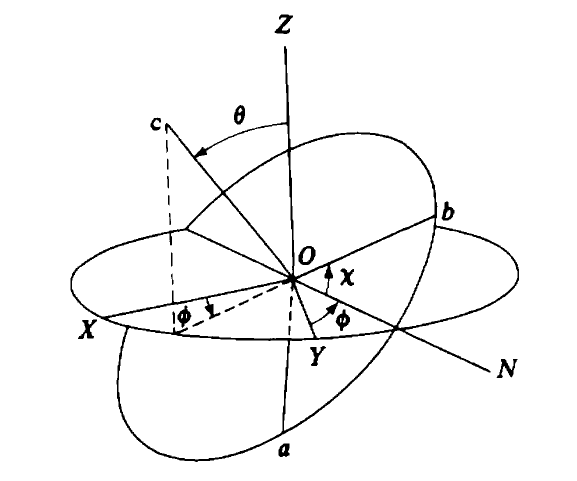
\includegraphics[width=0.4\textwidth]{Angulos_Euler.png}
\caption{Ángulos de Euler. }
\label{euler}
\end{figure}
$$
\hat P_{\phi}=-i\hbar\frac{\partial}{\partial \phi},\,\ \hat P_{N}=-i\hbar\frac{\partial}{\partial N},\,\ \hat P_{\chi}=-i\hbar\frac{\partial}{\partial \chi}
$$
\end{frame}

%DIAPOSITIVA 5
\begin{frame}{La molécula como un sólido rígido}
\framesubtitle{Pasamos a la cuántica}
Con un poco de trigonometría
\begin{equation*}
{\tiny\hat P_a = i\hbar \left[cos\chi csc\theta \frac{\partial}{\partial \phi} - cos\chi cot\theta \frac{\partial}{\partial \chi} - sin\chi \frac{\partial}{\partial \theta} \right]}
\end{equation*}
\begin{equation*}
\tiny\hat P_b = i\hbar \left[-sin\chi csc\theta \frac{\partial}{\partial \phi} + sin\chi cot\theta \frac{\partial}{\partial \chi} - cos\chi \frac{\partial}{\partial \theta} \right]
\end{equation*}
\begin{equation*}
\tiny\hat P_c = -i\hbar \frac{\partial}{\partial\chi}
\end{equation*}

O también:

\begin{equation*}
\hat P_X = i\hbar \left[cos\phi cot\theta \frac{\partial}{\partial \phi} - cos\phi csc\theta \frac{\partial}{\partial \chi} + sin\phi \frac{\partial}{\partial \theta} \right]
\end{equation*}
\begin{equation*}
\hat P_Y = i\hbar \left[sin\phi cot\theta \frac{\partial}{\partial \phi} - sin\phi csc\theta \frac{\partial}{\partial \chi} - cos\phi \frac{\partial}{\partial \theta} \right]
\end{equation*}
\begin{equation*}
\hat P_Z = -i\hbar\frac{\partial}{\partial\phi} 
\end{equation*}
\end{frame}

%DIAPOSITIVA 6
\begin{frame}{La molécula como un sólido rígido}
\framesubtitle{¿Cómo obtenemos las autofunciones y autoenergías del hamiltoniano?}
\begin{itemize}
\item	Sustituiyendo $\hat P_a$, $\hat P_b$ y $\hat P_c$ en $\hat H_{rot}$ y resolviendo la ecuación de autovalores \ding{55}
\item Usando relaciones de conmutación \ding{51}
\begin{equation*}
\left[H_{rot}, \hat P^2 \right] = 0
\end{equation*}
\begin{equation*}
\left[H_{rot}, \hat P_J \right] = 0
\end{equation*}
\begin{equation*}
\left[H_{rot}, \hat P_c \right] = i\hbar \left(\frac{1}{2I_a}-\frac{1}{2I_b}\right)\left(\hat{P_a}\hat{P_b}+\hat{P_b}\hat{P_a}\right)
\end{equation*}
\end{itemize}
Lo que nos da 
\begin{equation}
\hat H\psi = E\psi
\end{equation}
\begin{equation}
\hat P^2\psi = J(J+1)\hbar \psi, \qquad J=0,1,2...
\end{equation}
\begin{equation}
\hat P_Z\psi = M\hbar\psi, \qquad M = 0,\pm 1,...,\pm J
\end{equation}
\end{frame}

%DIAPOSITIVA 7
\begin{frame}{Rotor rígido cuántico: Estados propios y autovalores}
\framesubtitle{El rotor esférico $I_a=I_b=I_c= I$}
La ecuación de Schödinger es:
\begin{equation*}
\frac{\hat P^2}{2I} \psi = E\psi
\end{equation*}
Resolviendo la ecuación obtenemos que:$$\frac{1}{2I}J(J+1)\hbar^2\psi=E\psi$$
\begin{equation}
E=\frac{J(J+1)\hbar^2}{2I}, \qquad J=0,1,2...
\end{equation}
En este caso, tenemos además que
\begin{equation}
\left[\hat H,\hat P_c \right]=0
\end{equation}
con $$\hat P_c \psi = K\hbar\psi, \qquad K = 0, \pm 1,..., \pm J$$
Luego la energía está $(2J+1)^2$ veces degenerada.
\end{frame}

%DIAPOSITIVA 8
\begin{frame}{RRotor rígido cuántico: Estados propios y autovalores}
\framesubtitle {El rotor simétrico: $I_a=I_b\neq I_c$ (caso achatado) o $I_a\neq I_b=I_c$ (caso alargado)}
\end{frame}


\end{document}